% $Id: DELayout_implnotes.tex,v 1.1 2004/06/09 12:32:20 theurich Exp $

%\subsection{Design and Implementation Notes}

The DELayout class provides an additional layer of abstraction on top of the virtual machine (ESMF\_VM) layer. There are three key aspects the DELayout class deals with.

\begin{enumerate}

\item Problem decomposition via logical {\it decomposition elements} (DEs).

\item Support of load balancing in terms of computational and connection weights on and between the DEs. 

\item Mapping of the logical problem decomposition onto an ESMF virtual machine.

\end{enumerate}

%\begin{center}
%\scalebox{0.6}{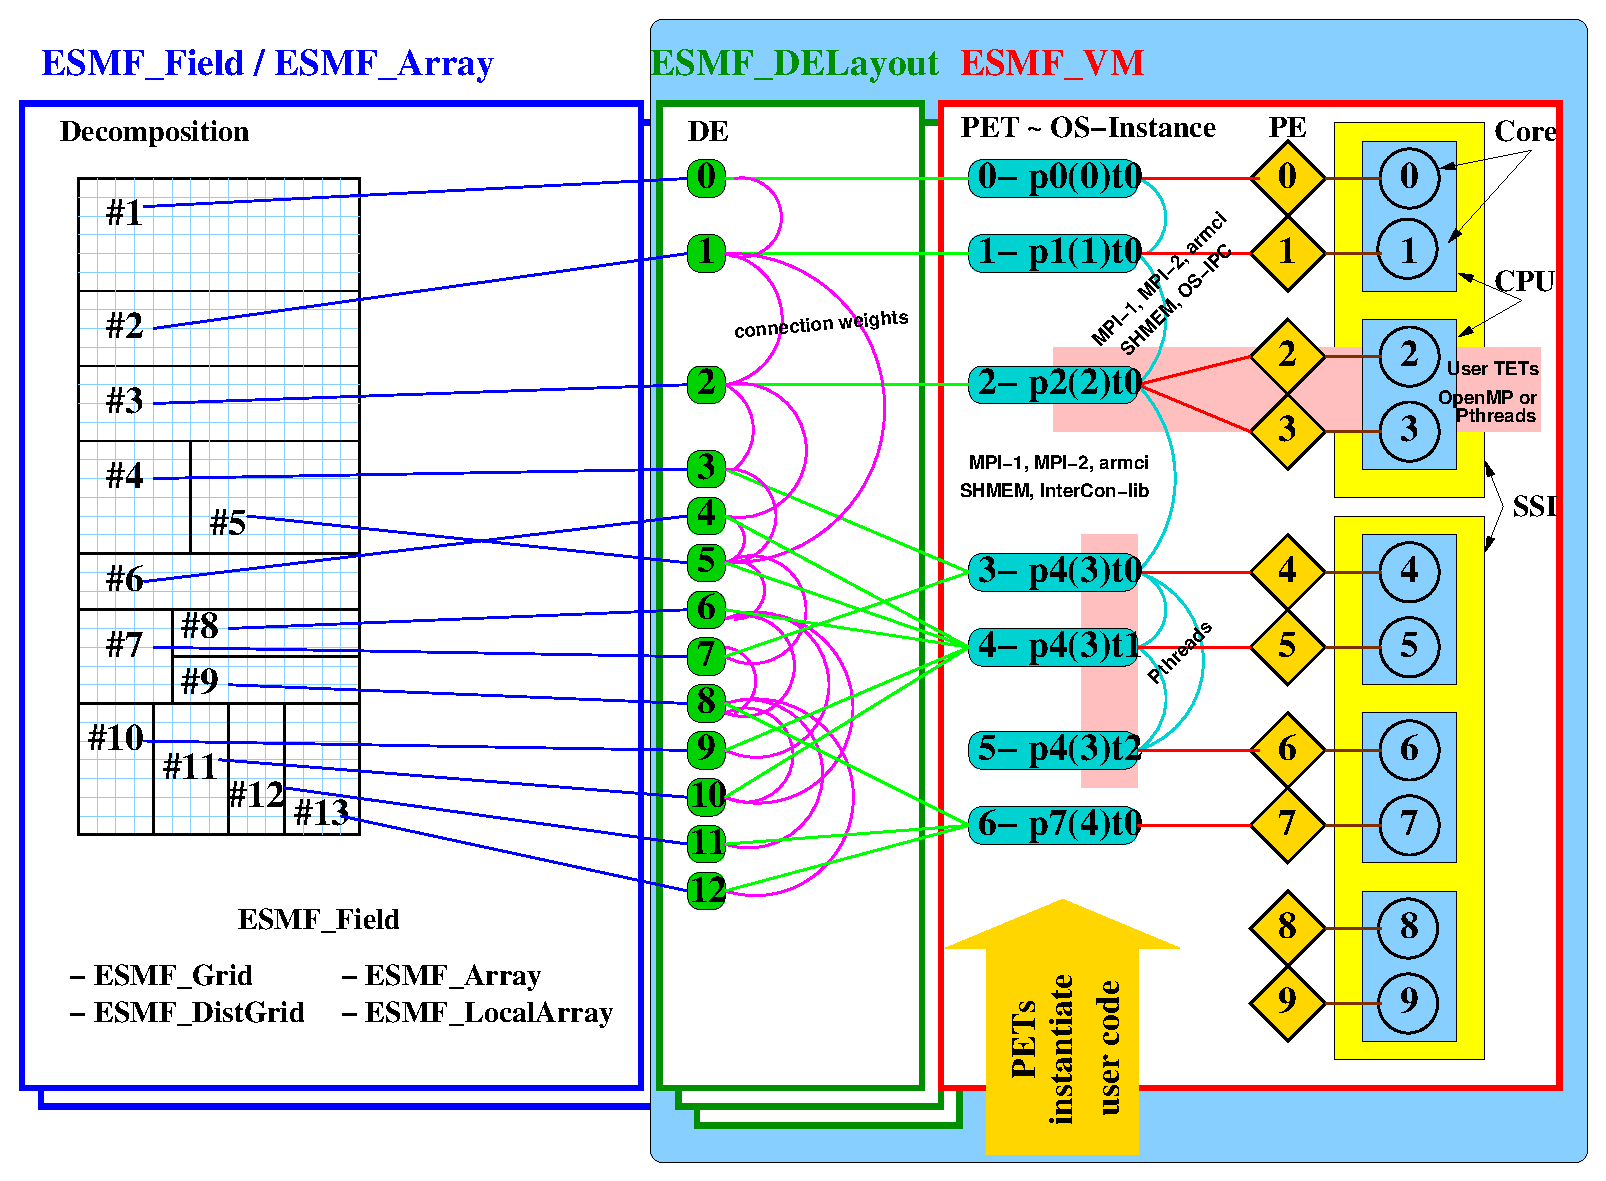
\includegraphics{VM_design.eps}}
%\end{center}


{\bf Definition of terms used in the diagram}

\begin{itemize}

\item DE: Decomposition element.

\end{itemize}
